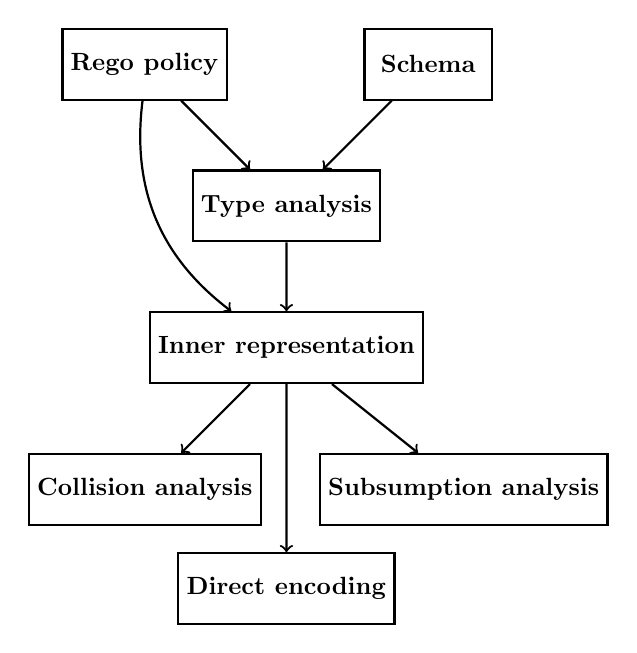
\begin{tikzpicture}[
            s/.style={draw,thick,rectangle,minimum height=10mm, minimum width=18mm},
            % code/.style={draw,fill=blue!10,rectangle,minimum height=10mm, minimum width=18mm,rounded corners=2mm},
            e/.style={fill=gray!50},
            xsh/.style={xshift=15mm},
            transform shape, scale=0.9
        ]

        \tikzset{
            node distance=20mm,
        }

        \node[s] (input) {\textbf{Rego policy}};
        \node[right of=input] (e) {};
        \node[s,right of=e] (schema) {\textbf{Schema}};
        \node[s,below of=e] (ta) {\textbf{Type analysis}};
        \node[s,below of=ta] (ir) {\textbf{Inner representation}};
        \node[below of=ir] (e2) {};
        \node[s,left of=e2] (ca) {\textbf{Collision analysis}};
        \node[s,below of=e2,yshift=6mm] (enc) {\textbf{Direct encoding}};
        \node[s,right of=e2,xshift=5mm] (sa) {\textbf{Subsumption analysis}};

        \draw[->,thick]
            (input) edge (ta)
            (schema) edge (ta)
            (input) edge[bend right] (ir)
            (ta) edge (ir)
            (ir) edge (ca)
            (ir) edge (enc)
            (ir) edge (sa)
        ;

\end{tikzpicture}
